\chapter{DISCUSSION}
In this thesis I have described a number of methods that I developed and implemented to optimize reduced neuron models against experimental data collected from real neurons.
I then verified that this optimizer works in the sense of being able to recover ground truth models given only simulated data from those models.
I showed that successful optimization depends upon certain characteristics of the experimental data and the features extracted from it, and identified a flaw in the approach of optimizing against aggregated data from neural populations. 
I demonstrated that the optimizer does an adequate job at fitting reduced neuron models to real experimental data from single neurons, and that certain models (and cell types) are easier to optimize than others.
I showed that published models differ from the experimental data they ought to be explaining, on which features they differ most, and I show proto-typed analysis pathway that is capable of demonstrating if and when optimized models can better match experimental data, compared to other published models.
%and that it is possible to optimize these models to better match those experimental data.
Finally, I presented a tool to bring this optimization framework to the masses.

\emph{Efficient} optimization of reduced neuron models is significantly non-trivial, as an alternative, obtaining merely satisfactory biologically plausible models is several degrees easier.
Below I provide a number of examples of optimization pitfalls which were not obvious at the start of my research, but which I discovered during my research, and which were on ongoing source of confusion, not just for me, but for my whole research team.
I believe that it is important to share these conceptual traps with my readership, including those who may wish to continue such optimization work.

\section{What is Required for Successful Optimization?}
For optimization to both succeed and be useful, several criteria must be met \citep{van2007neurofitter}:
\begin{itemize}
\item Relevance: The objective function should reflect fundamental and important properties of the data that a good model would reproduce.
\item Speed: The objective function should be fast to calculate, since typically a large number (potentially millions) of evaluations are performed during the search, many of which may require re-simulation of the model.
\item Efficient Convergence: The solution space should be as continuous and convex as possible, so that the search algorithm can rapidly converge to a global optimum.
\end{itemize}

%The EFEL signal processing suite was able to produce measurements that fulfilled the speed criteria. 

\subsection{Relevance of the Objective Function}
\subsubsection{Source of Data Constraining the Objective Function}
Due to the abundance and diversity of data available through the NeuroElectro Project \cite{tripathy2014neuroelectro}, my initial work relied heavily on that data source.
However, that data is enriched in passive membrane properties as well as the details of individual action potential waveforms.
But what distinguishes, say, a Layer 5 pyramidal cell in motor cortex from a Layer 5 pyramidal cell in visual cortex, in terms of the computational principles that systems neuroscientists might care about (e.g. decoding, information, etc.) is more likely to be reflected in the patterns of spiking and not the dynamics of single spikes or subthreshold behavior.
Furthermore, most reduced models are not implemented in way that allows for richly detailed action potential waveforms to be reproduced.

Together, this implies that reduced models optimized against data exclusively from NeuroElecto may be the worst of both worlds: they fail to capture the sub-millisecond dynamics of the action potential encoded in that data, while also failing to exhibit any of the suprathreshold dynamics (e.g. types of bursting) that distinguish one cell type from another, in the mind of a systems neuroscientist.
This problem is mitigated by including complementary data sources (like the Allen Cell Types database) that can address these dynamics.
Future optimization efforts should take care to identify the data sources that capture the dimensions of the experimental data along which meaningful differences between cell types can be resolved, and which models are rich enough to express.

\subsubsection{Number of Components in the Objective Function}
Theoretically every additional component included in the objective function--every constraint derived from some experimental feature--should make the error surface a better answer to the question, ``Is this a realistic model of the neuron of interest?".
Although they might increase the computation time required per objective function evaluation, such additional components may rapidly exclude large volumes of parameter space from unnecessary exploration.
For example, when modeling a bursting neuron, including burst-statistics as one of the features under evaluation will quickly exclude non-bursty regions of parameter space from consideration.

And yet a successful optimization recipe should not naively involve the use of all available computable features.
Some features might be biologically irrelevant, or impossible for some model class to reproduce, or have extremely discontinuous error surfaces.
This makes the task of optimization less automatic--careful human guidance is needed to curate the appropriate features for the task. 

\subsection{Speed of Optimization}
\subsubsection{Speed of the Objective Function}
A large fraction of the compute cycles spent evaluating each parameter set are expended on identifying the rheobase current, thus unlocking the calculation of several subsequent measurements.
Fortunately, for slower model implementations this can be sped up significantly through parallelism, as described in section \ref{sec:parallel-rheobase}.
In some applications, parallel code scheduling is incompatible with with the just-in-time (JIT) compilation approach described in Section \ref{sec:new-models}, so parallelism sometimes trade off against raw model simulation speed. 

\subsubsection{Speed of Parallel Exploration}
In this work it was sometimes memory pressure and not clock speed that produced the major bottleneck.
This was especially true when mining features from pre-existing databases.
In these contexts I made use of a delayed iterator provided by the Dask library Dask \citep{rocklin2015dask} to stream very large amounts of data in memory-friendly chunks as needed.
Delayed evaluation using the Dask library also resolved conflicts Additionally delayed evaluation caused fewer conflicts with JIT code.
%timlyness of results was not the fundamental 
%Additionally the dask delayed algorithm
%In this context there were two different classes of model: 
%Models that should have parallel Rheobase or parallel chromosome evaluation.

%Caching of simulation results can also speed up evaluation, for example when computing multiple features based upon the same simulated membrane potential trace (e.g. spike count and time to first spike at a given current amplitude).
% Although this is an obvious opportunity for speed up, it was abandoned as the first pass attempt at solving this inside Neuronunit lead to unpredictable bugs for the whole team of programmers involved. This would probably work in current versions of neuronunit.
%XXXX More about speed here.




%\subsection{More about Rastrigin's function...?}
%Rastrigin's function has convexity in two scales. On the larger scale the surface %has a convex property, on the small scale the function is uniformly pocked with %minima wells. In order for the GA to optimize Rastrigin's function it must be %able to exploit the global information of the error surface, and simultaneously %the genes will often converge for generations in the minima, but they won't get %stuck there for two reasons: Reason 1, the global convex shape will be %represented in some genes that participate in cross over, therefore it is %learnable. Reason 2:
% mutation and cross-over provide a significant repulsive force, driving %chromosomes to test other locations despite that they perceive those locations to %be less optimal.\\
   %\begin{figure}
  %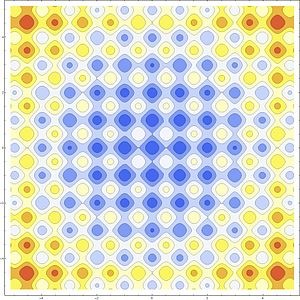
\includegraphics[]{figures/rastagrind.jpg}
  %\caption{}
   %\end{figure}
   
%   It is worth noting that although Rastrigrins function is challenging it does not the present the worst gradient to learn from. Worse than Rastrigrins function, are functions that on a large scale are flat, but on the smaller scale contain a high density ripples.
%   but lacks this global convex trend, excepting for an abrupt and localised descent to the optima.
   
%   Without some first prior knowledge of the error surface, a likely outcome is to attempt optimize on uninformative surfaces. If an uninformative surface is applied, it does not mean that the genetic algorithm will not succeed, it only means that the performance of the GA may be only marginally better than random sampling, or exhaustive search of the error surface.
   %Random sampling, sounds bad, however, if the best random solution is digitally stored, and the number of samples applied is less than the possible number of samples in an exhaustive search, random sampling may better resolve the exploitation/exploration dilemna than both gradient descent, and exhaustive search.
 

   
  

\section{Sensitivity to Error Surface Quality}
In the spirit of the list above provided by \cite{van2007neurofitter}, the next item should be called ``Efficient Convergence", but this efficiency really comes down to the nature of the error surface created by the choice of models, tests, and experimental data.

\subsection{Objective Function Dimensionality vs Model Parameter Dimensionality}
If a given class of models is capable of describing the behavior of a given real neuron, then the number of independent, reliable tests used to generate the objective function can be as large as desired; more tests just provide more information to quickly rule out irrelevant regions of parameter space.
On the other hand if a model class is only capable of describing a fraction of the real neuron's behavior, too many distinct tests will result in an optimization problem that can never be fully satisfied.
Since ``all models are wrong, but some are useful" (Box, 1976), let us imagine that we usually in the latter case.

\subsection{When Does Genetic Optimization Get Stuck?}
Genetic algorithms are known as derivative-free optimizers, since they do not follow any gradient down the error surface, or even know of the existence of such a gradient.
Chromosomes only survive and reproduce differentially according to their location on the error surface.
Thus, genetic optimization is never truly "stuck" inside a local minima on the error surface, as mutation or crossover can always produce new chromosomes outside the basin of attraction.
Despite this robustness, just like in gradient descent, genetic algorithms can only be guided by information in the error surface.
When the objective function has a low-dimensionality, for example when it is based upon tests that mostly compute small variations on the same small number of features of the simulation output, it may not provide enough information to distinguish one location in parameter space from another one close by, even though the first may be closer to the optimal solution than the second.
In other words, many regions of parameter space may be locally flat at a mesoscopic scale, and local minima at a microscopic scale may thus be difficult to escape.
No lower error solution may be available within a reasonable distance (in parameter space) from the current one.
A variety of potential error surfaces are presented in Figure \label{fig:test2}.

\begin{figure}
\centering
      \label{fig:test1}
      \centering
      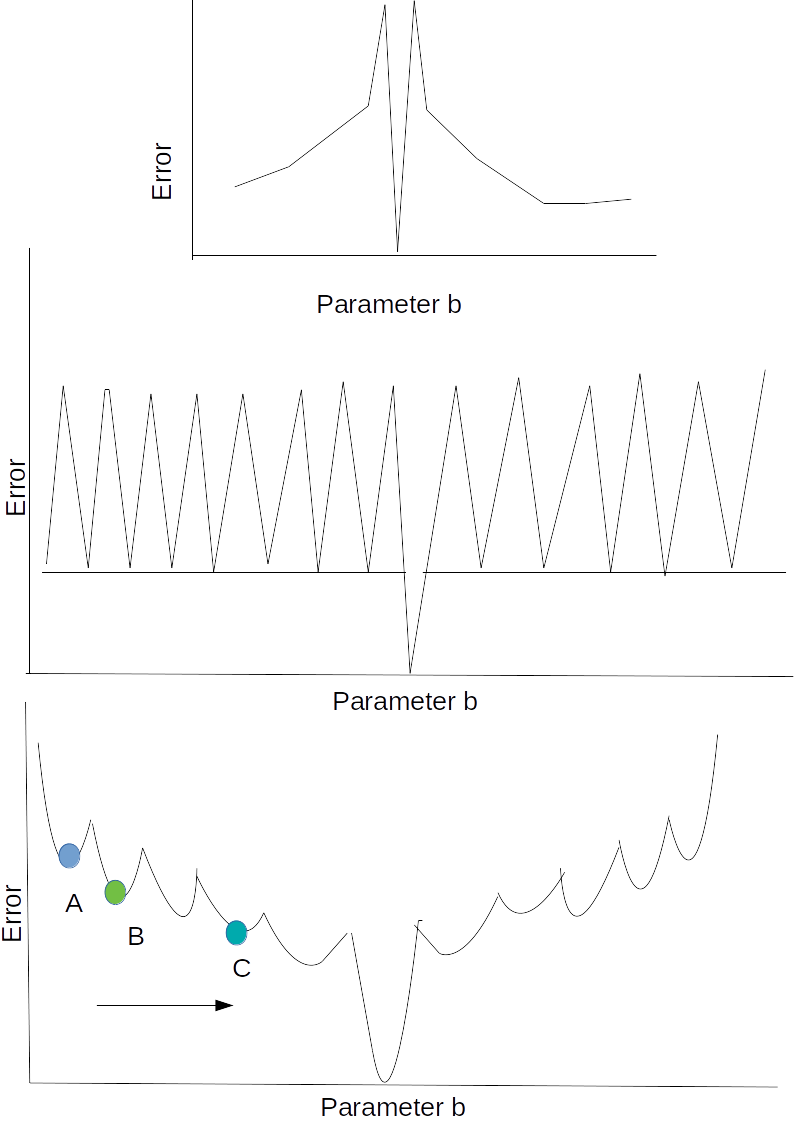
\includegraphics[scale=0.75]{figures/spectrum_worst_error_surfaces_error.png}
      \caption[Challenging Error Surfaces]{\textbf{Challenging Error Surfaces}. 
      Fitness here should be relabeled "Error".
      The top panel shows an error surface where an optimizer is unlikely to identify the global minimum error.
      Any exploration of the region leading towards that minimum is likely to be abandoned prematurely.
      Only an extremely lucky set of initial chromosomes or a random mutation might result in exploration of the region immediately around the global minimum.
      The middle panel is more hopeful, showing an error surface that does not actively block the global minimum from being explored.
      However, the surface is still mostly uninformative.
      The bottom panel shows a cross-section of Rastrigrin's function (described in the Introduction).
      Despite its hype, this is really the least challenging of the three error surfaces shown here, as there as at least long-range structure to the error surface that a genetic algorithm can exploit.
      }
      \label{fig:test2}
\end{figure} 

\subsection{Defects in the Error Surface}
The real error surfaces that guide optimization here have ``defects", for example discontinuities (due perhaps to bifurcations in the underlying dynamical system, e.g. from spiking to non-spiking) or to deep local minima, that make optimization challenging.
I coined the term ``corrugated" to describe surfaces low amplitude oscillatory disturbances across the error surface.

Some optimization techniques require a perfectly convex error surface to converge.
Genetic algorithms are more tolerant, up to a point, but an extremely high dimensional optimization problem with a large number of optima can still be intractable.
So which error surface defects are truly harmful?
This largely comes down to scale.
The corrugation observed in the error surfaces here was typically on a much smaller scale than the long-range structure that guides optimization.
Consider something analogous to a signal-to-noise ratio (SNR), describing the information that guides optimization vs the wrinkles that impede it.
When SNR is larger, defects are less consequential.
Figure \ref{fig:easy-case} gives an example of an error surface that, while not totally continuous or convex, is nonetheless easily handled by the optimizer.

\begin{figure}      
\centering
      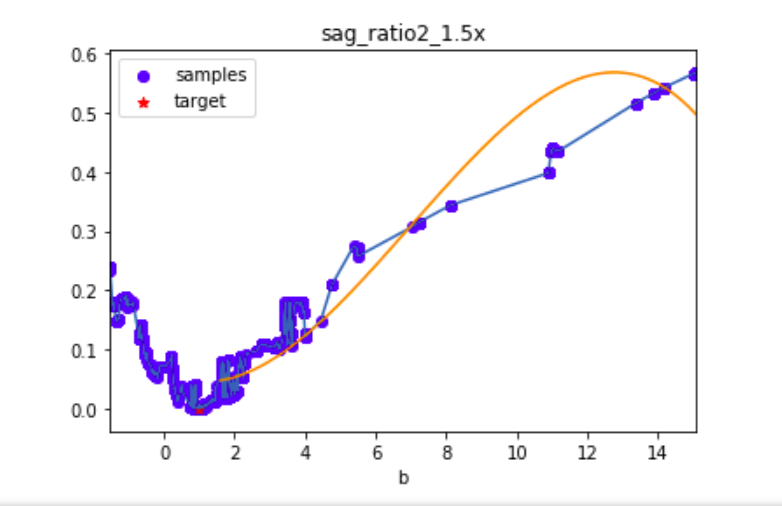
\includegraphics[scale=0.85]{figures/parameter_b_friendly_surface.png}
      \caption[A Non-convex but Manageable Error Surface]{\textbf{A Non-convex but Manageable Error Surface}.
      The vertical axis shows error (model-data disagreement) for ``sag-ratio" feature computed at 1.5 $\times$ rheobase as the value fo the $b$ parameter in the Izhikevich model is slowly varied.
      The blue dots show the actual error values, and the orange curve shows a low-order polynomoial regression fit.
      While the fit is clearly not perfect, the fact that the error surface can be approximated by a low-order polynomial suggests that it will not be difficult to find the minimum (red dot).}
      \label{fig:easy-case}
\end{figure}

I observed that the NSGA2 selection algorithm was particular vulnerable to defects in the error surface, and required a higher SNR to obtain optimal solutions.
NSGA2 is a fundamentally conservative and short-range approach to evolution, so it may simply lack the drive to escape problematic regions of the error surface.
Unlike NSGA2, IBEA was less sensitive to such defects, and required a lower SNR to converge rapidly. 

However, in any algorithm as the optimum is approached, the rate of mutation must slow down to enable efficient short-range exploitation of the peri-optimum region.
one should not expect to see evidence of efficient-learning. In later phase of learning when the optimizer will be more sensitive to small amplitude corrugations, which become large relative to the smaller improvements of error.
%to by moving between, say, a parameter set $1\%$ away from the optimum and the optimum itself.

The multiobjective function is derived from the objective functions associated with each feature used in optimization.
As such, the multiobjective function will be more corrugated if more of the component objective functions are corrugated.
Consequently, optimization is more likely to converge if the number of corrguated components is kept to a minimum.
In practice, I observed satisfactory solutions even when only $>\frac{1}{2}$ total number of objectives had no corrugation.
For example, in a four-objective problem, if the $4$th objective is uninformative, but not actively misleading, inclusion of that 4th objective may only slow down the speed of optimizer convergence, but not actually change the final outcome.
By contrast, if that $4th$ objective is actively misleading, the optimizer will likely find a satisfactory (but non-optimal) solution by compromising with the dominant $3$ objective functions.

%\begin{comment}
%\begin{figure}
%\begin{center}
%     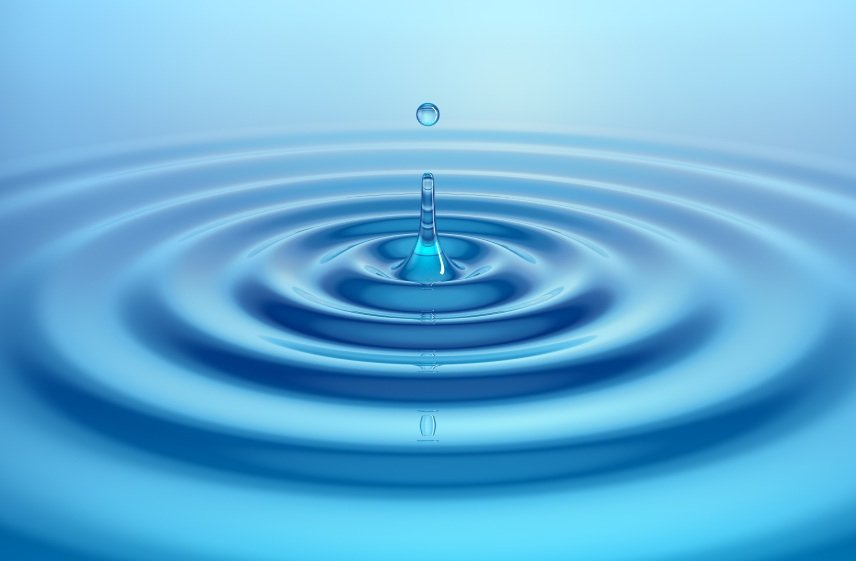
\includegraphics[scale=0.65]{figures/pond_ripple_surface.png}
%     \caption[Conceptualizing moderate to worst case error surfaces]{In the case of pond ripples the cost function is defined so that the maxima is the optimal %location on the surface. Ripples on a body of water are more challenging to optimize, as the water surfaces are approximately flat on the large scale, yet on the small scale maximas will be temporary preoccupy the GAs learning, but outside of those peaks, there is little large scale information to utilize.}
%      
%      \label{fig:test1}
%\end{center}
%
%\end{figure}
%\end{comment}



% Note Help wanted making a professional version, of this known to be unattractive draft/concept figure.
     
      % The second type of error surface actually a 1D (and upside down) cross section of the 2D pond diagram, only actively misleads locally, globally it simply contains no helpful global information. Learning will not be of any assistance in obtaining the optima, but also learning won't be a disadvantage either, the Genetic Algorithm, will simply behave as a random sample testing algorithm, the GA will find the optimum in time, but possibly not as quickly or reliably as exhaustive search would. The second figure is a cross section of the pond ripple argument}







%   When considering 2D relationships between single parameters and single objective functions, ideally each error function might contribute helpful information, which en-masse boosts the total amount of helpful information. For-instance some 2D error mappings, may contain one or more local minima, but in the same region a different error mapping could lack the error well, meaning that at least one out of two error functions contribute incentive to stride across a minima. The mapping that contains wells, might still be useful to guide optimization, as it may also lack minima in regions were the counterpart has them, additionally the alternative mapping may have regions of $~0.0$ gradient where the other mapping contains significant gradient.
   
   % I am not sure if its impossible to make progress.
 %  Through strategy it is possible to optimize satisfactorily without complete prior knowledge of error surfaces, although such a strategy is not recommended. If prior knowledge of an error surface is prohibited, evolutionary algorithms are definitely a more likely to work than gradient descent.
   
   
   % I don't know if this is true:
   % through good luck you could do heaps of optimization, whithout knowing the error surface.
   % It is almost impossible to make progress without some prior knowledge of the error surfaces, as knowledge of the error surface is a prerequisite for constraining optimization. 
   
%   Not all surfaces, provide equally useful information. There are spectrum's of surface quality between convex triangular or parabolic depressions acting as the best solution surfaces, flat functions, and misleading functions. 
   
\subsection{Contingent Discontinuities}
\label{sec:contingent_discontinous}
Some tests used to compute the objective function may depend on the results of other tests.
They may depend on the measured value of one feature, for example, a test of the action potential width at half-height depends on the height measured from threshold which depends on the threshold.
Or they may depend on a stimulus parameter derived from a previous test; for example, computing the first inter-spike interval (ISI) at 1.5x rheobase first requires computing rheobase, and then multiplying the rheobase value by 1.5 to generate the stimulus for the ISI test.
Such an ISI test--and its results--is thus ``contingent" on the results of the rheobase test.
This has confounding implications.
Suppose that as some model parameter $X$ is increased, the cell becomes more excitable.
All things being equal, more excitability would be associated with a lower rheobase, and with a narrower first inter-spike interval at a fixed current.
But because the rheobase determines the value of the actual current injected in the ISI test (i.e. the ISI test is contingent), the ISI could go up or down; it would go down if the direct effect of greater excitability associated with increased $X$ dominates; it would go up if the indirect effect of a smaller current injection dominates.
In fact, it is impossible (or at least impractical) to predict which of these will "win", and the resulting error surface for the ISI test becomes extremely corrugated, as small increments in $X$ cause increases and then decreases in the error of the objective function, with no discernible pattern.

\subsubsection{Examples of Contingent Discontinuities}
Figure \ref{fig:probably_smooth_constraint} provides a concrete example of the discontinuous error surface that results from such contingencies.

\begin{figure}
\centering
      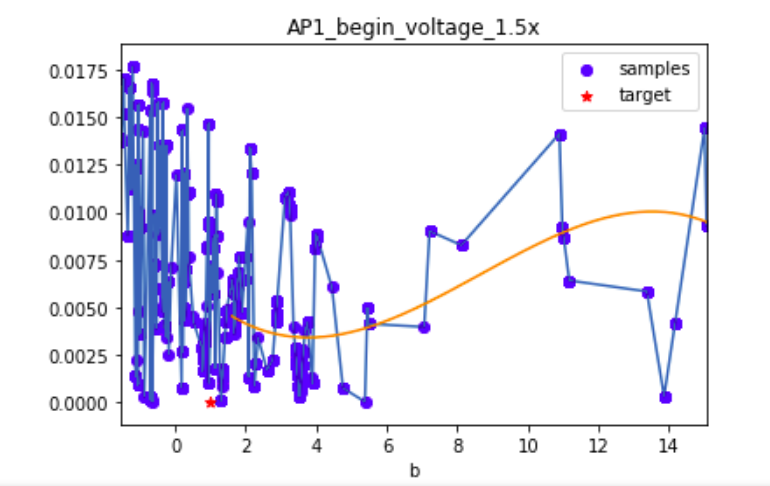
\includegraphics[scale=0.85]{figures/parameter_b_hopeless_surface.png}
      \caption[A Non-convex and Unmanageable Error Surface (1)]{\textbf{A Non-convex and Unmanageable Error Surface}.
      Similar to Figure \ref{fig:easy-case}, but showing the error in another feature (the membrane potential at the start of the AP waveform) as the same parameter is varied.
      This error surface is extremely corrugated, the polynomial fit has no hope of approximating what is going on for $b<6$, and the optimizer stands little change of finding the global minimum, if such a minimum is even meaningful here.
    }
      \label{fig:probably_smooth_constraint}
\end{figure}

The problem is even more extreme when the contingent test can produce missing values.
For example, an ISI test depends on their being an inter-spike interval to measure, i.e. it requires a second spike to be produced.
If there is no second spike, this test will emit a missing value.
Thus as $X$ is increased, the error surface associated with the ISI test will be pocked with missing values every time the underlying change in excitability is offset too much by the ensuing change in rheobase-derived injected current.
An example of this even more challenging case is given in Figure \ref{fig:discontinuous_constraint}.

\begin{figure}
      \centering
      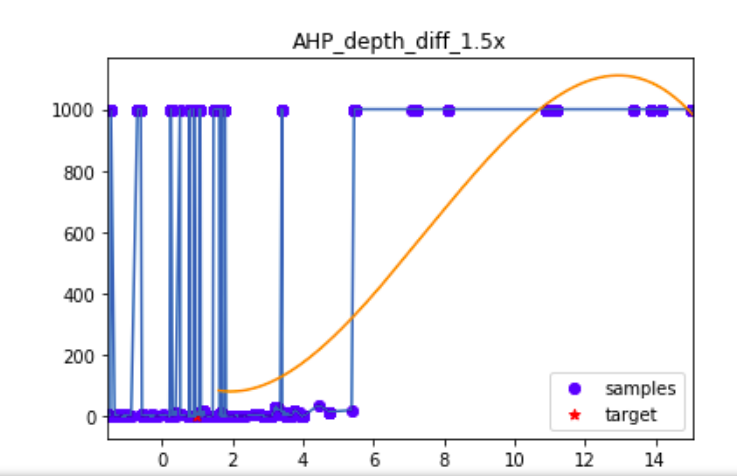
\includegraphics[scale=0.85]{figures/parameter_b_hopeless_surface2.png}
      \caption[A Non-convex and Unmanageable Error Surface (2)]{\textbf{Another Non-convex and Unmanageable Error Surface}. Similar to Figure  \ref{fig:probably_smooth_constraint}, but now for differences in the depth of the after-hyperpolarization across repeated spikes.
      This feature is actually uncomputable for some values of the parameter $b$ varied along the x-axis, because as this parameter changes, the rheobase changes, and the number of spikes observed at the rheobase varies between 1 and 2.
      When the number of spikes is 1, any parameters that describes differences across spikes is undefined.
      Because the optimizer cannot work with missing data, a very larger error (1000) is imputed.
      However, this means that it is nearly impossible to identify the global minimum, because many promising chromosomes mutate onto the peaks of the error surface and do not make it into subsequent generations.
      A genetic algorithm sees the region $b<6$ as essentially random.}
      \label{fig:discontinuous_constraint}
\end{figure}

\subsubsection{Causes of Contingent Discontinuities}
And an error surface plagued with too many missing values is essentially unusable.
These contingent discontinuities present a major problem to the logic of contingent testing that underlies most of the optimization presented here.
I verified that the reasoning above was matched by the observed changes in simulated behavior in response to changes in model parameters.
I found that slowly varying a single model parameter in a reduce model can cause two extracted features to vary inconsistent ways (Figures \ref{fig:corrugation-cause-1} and \ref{fig:corrugation-cause-2}).

\begin{figure}
\begin{center}
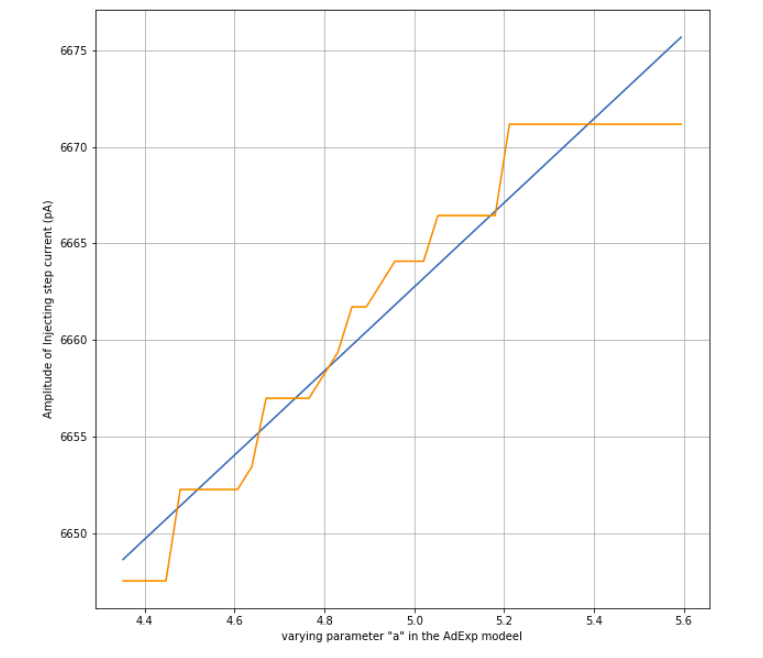
\includegraphics[]{figures/fundamental_cause_of_corrogations.png}
\caption[Causes of Corrugation (1)]{\textbf{The Causes of Corrugation in Error Surfaces: Part A}.
I identified the main cause of corrugated error surfaces by re-calculating feature values as single parameters were varied.
Here, I vary parameter $a$ in the AdEx model.
The orange trace shows the computed rheobase current as this parameter is varied.
Note that it grows in a step-like manner, not according to the smooth linear fit (blue).
During periods when the rheobase is not increasing (but the parameter value is), the parameter may cause some other feature, computed at the current that causes 14 spikes to fire to vary in one direction.
Once the 14 spike current jumps, the stimulus used to compute the feature has changed, so that same feature may vary in the other direction.
Consequently, a computed feature-value may zig-zag, rather than exhibiting a smooth change, as a parameter is varied.}
\label{fig:corrugation-cause-1}
\end{center}
\end{figure}

In Figure \ref{fig:corrugation-cause-2}, I show a more concrete example of the same phenomena.
\begin{figure}
\begin{center}
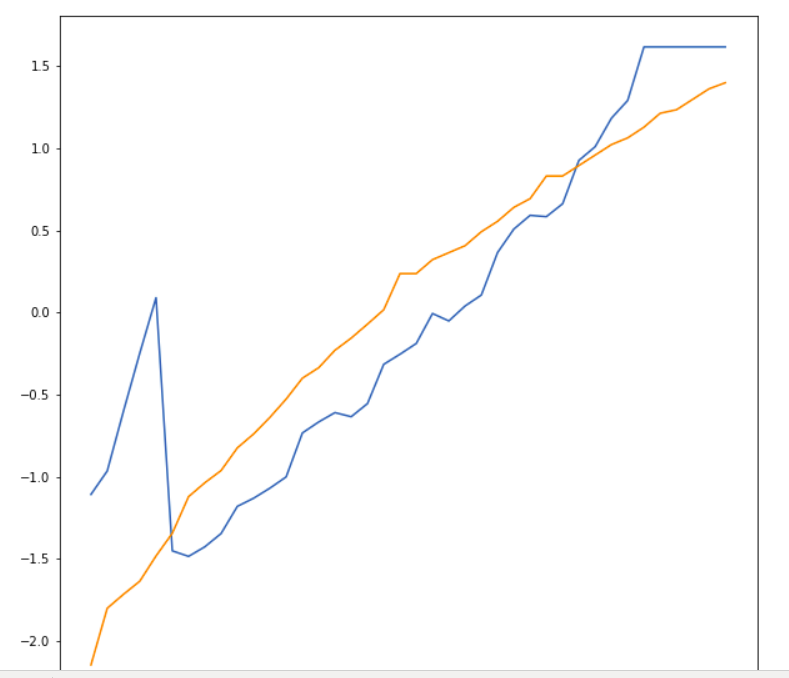
\includegraphics[]{figures/rh_vs_vt.png}
\caption[Causes of Corrugation (2)]{\textbf{The Causes of Corrugation in Error Surfaces: Part B}.
Using an Izhikevich model, I vary a single odel parameter ($a$) as in Figure \ref{fig:corrugation-cause-1}, and plot the rheobase current (orange, normalized to its mean value) but also compute the value of the spike threshold (blue, also normalized).
Note the non-linear behavior of the response of this feature value to the change in the model parameter.
This non-linear behavior is mainly driven by a change in the amplitude of the injected current used to evoke it (the rheobase current), and not to underlying non-linearity in the location of the spike threshold for a fixed current.}
\label{fig:corrugation-cause-2}
\end{center}
\end{figure}

This can also be visualized in the waveforms themselves.
In Figure \ref{fig:variable-vt} the location (in time) of the threshold relative to the peak of the action potential varies in unpredictable ways as a single parameter of the model is increased.

\begin{figure}
\begin{center}
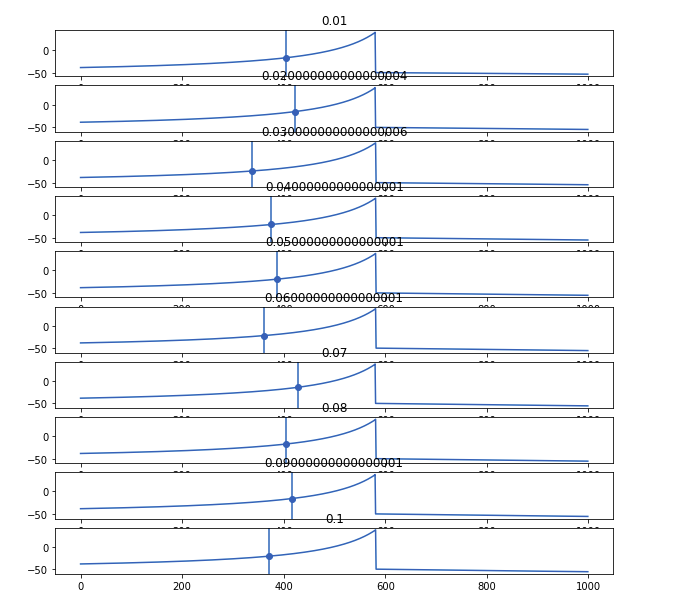
\includegraphics[]{figures/variable_vt.png}
\caption[Causes of Corrugation (3)]{\textbf{The Causes of Corrugation in Error Surfaces: Part C}.
In order to see this effect directly in the responses themselves, I plot the action potential waveforms for the Izhikevich model as the value of parameter $a$ increases in small steps from the bottom panel to the top panel.
At each value of this parameter, rheobase is computed and the waveform of the spike evoked at rheobase is extracted.
Each such spike is aligned across panel, so that differences in the lead up to that spike can be examined.
The spike threshold, identified by the moment when the slope of the membrane potential reaches a target value, is shown with each blue dot, and the time that the threshold is reached is indicated by each vertical line.
It is clear that while the time of the threshold changes as $a$ is varied, it does not do so systematically.
Therefore the resulting error surface will not be useful for optimization.
This demonstrates that making features contingent upon the responses to the rheobase current results in major challenges to optimizaton.}
\label{fig:variable-vt}
\end{center}
\end{figure}

%An izhikevich model is used to examine the effects of sweeping across changes to parameter 'a' while retaining all other paramters as constant, on the plot, rheobase is and $V_{T}$ is calculated for each different value of 'a' and plotted on the same y-axis. It becomes apparent that rheobase (the orange trace) has minor zig-zags in its value, while $V_{T}$, has bigger and more significant zig-zags in its error, at this point all we have done is slowly varied and calculated $V_{T}$ but we have not plotted $V_{T}$ in relation to APs

% If all other conditions are favorable , as the remaining objective functions may have high fidelity; 

\subsubsection{Overcoming Contingent Discontinuities}
With sufficient care taken to avoid too many corrugations in the error surface,  optimization can still be viable.
However, this may mean discarding otherwise useful features that could in principle distinguish between competing regions of parameter space.
An alternative approach is to discard the rheobase entirely as a contingency,
making tests depend not on the rheobase value obtained from each parameterization of the model, but on the rheobase observed in the experimental data itself.
In other words, if the rheobase of the biological neuron is 100 pA, then the $1.5\times$ rheobase ISI test should be performed with a current injection of 150 pA, even if the rheobase of the current model parameterization is some entirely different value.

Another approach is to dispense with the rheobase entirely, and simply test using a fixed set of current amplitudes that span the suprathreshold portion of the F-I curve, e.g. 200pA, 350pA, and 500 pA for a typical neuron.
This seems extremely direct, but it in some cases it fails to explore the most interesting peri-threshold portion of the F-I curve, where the dynamics of single spikes contain a great deal of information about peri-threshold dynamics.
For example, an after-hyperpolarization that is visible after single spike at rheobase may become completely swamped by the combination of inward pipette current and sodium current at values of injected current that are high above threshold.

\subsection{Does a Genetic Algorithm Adequately Report the Contours of the Error Surface?}
The error surface is vast, corresponding to all possible combinations of parameters at infinite resolution.
Naturally, this is only sparsely and strategically sampled.
Consequently there is no guarantee that it is has been adequately explored, and that lower error parameter sets do not exist somewhere that the optimizer did not adequately explore.

Next I describe how to visibly ``clean" corrugations from the error surface when using an approach based on a small list of non-contingent errors vs an alternative approach using models whose measurements are contingent on parameter dependent current values.

For each model a current is found that forces the model to fire at 12 spikes. Although not the exactly the same as rheobase, the algorithm is structurally identical, and the problems are the same. When eliciting a pre-determined spike count for any model parameterization (1 or x). This algorithm has the same propensity as the rheobase algorithm to introduce small current excesses into readings of subsequent tests, in this case EFEL tests of spike train shape.
%Because the rheobase algorithm is essentially an algorithm that searches %multiples of the experimentally observed rheobase.
Figures \ref{fig:constant_current} and \ref{fig:real_problem_nontrivial_surface-1} below show error surfaces from each paradigm.
Each of these figures depicts a heatmap of a 2D cross-section of the error surface.
The sensitivity of the objective function to systematic changes (grid search) of two parameters, centered around the optimizer's own solution, was explored.
All other parameters were held constant at the optimal values.
This effectively depicts a cross-section of the error surface near that solution.

%Case 1, Izhikevich model at threshold virtual experiment. Constraints used:
%\begin{table}
%\begin{tabular}{c}
%    TimeConstantTest \\
%    RestingPotentialTest \\
%    InputResistanceTest \\
%    CapacitanceTest \\
%    FITest \\
%\end{tabular}
%\caption[Izhikevich model rheobase constraints]{}
%\label{izhi-rheobase-constraints}
%\end{table}

%The surface plot from the supra threshold paradigm shows more contrast for two reasons: 1, it has less intermediary values (light green colour), reason two, it less high frequency changes, or ripples in the error surface.  

\begin{figure}
    \centering
    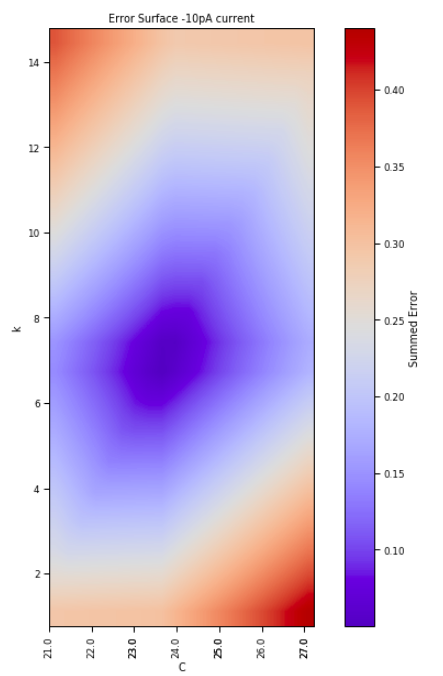
\includegraphics[scale=0.7]{figures/friendly_error_surface.png}
    \caption[Constant Currents Produce Tractable Error Surfaces]{\textbf{2D Cross-section of the Error Surface for an Izhikevich Model with No Contingent Tests}.
    The model was optimized against simulated data using 5 features.
    Any other features whose calculation is contingent on the rheobase were deliberately excluded.
    A 2D grid search was then applied (for parameters $C$ and $k$) around the resulting optimal set of parameters in order to visualize the local error surface.
    Although only 2 dimensions are explored here, there is no evidence of corrugation in this error surface, indicating that manageable, convex error surfaces can be realized when contingencies are removed.}
    \label{fig:constant_current}
\end{figure}

%\begin{figure}
    %\centering
 %   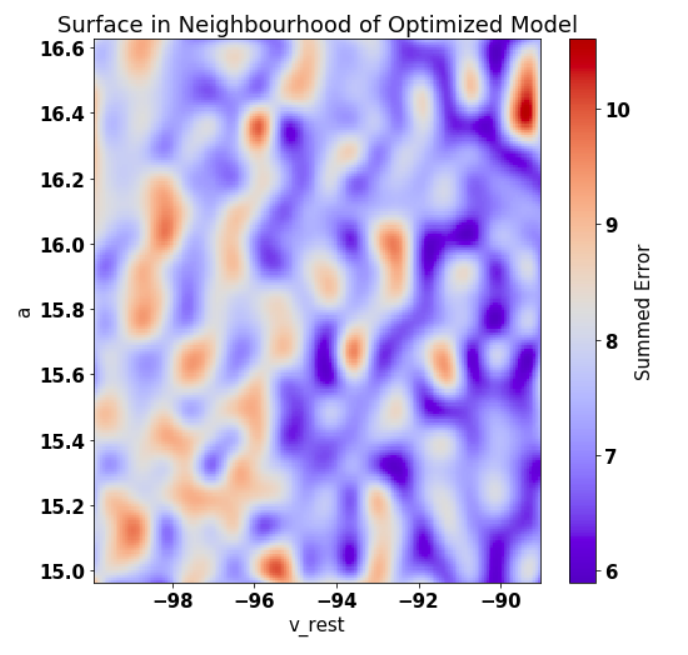
\includegraphics[scale=0.75]{figures/corrogated_surface_but_functional.png}
%\end{figure}  
\begin{figure}
    \centering
    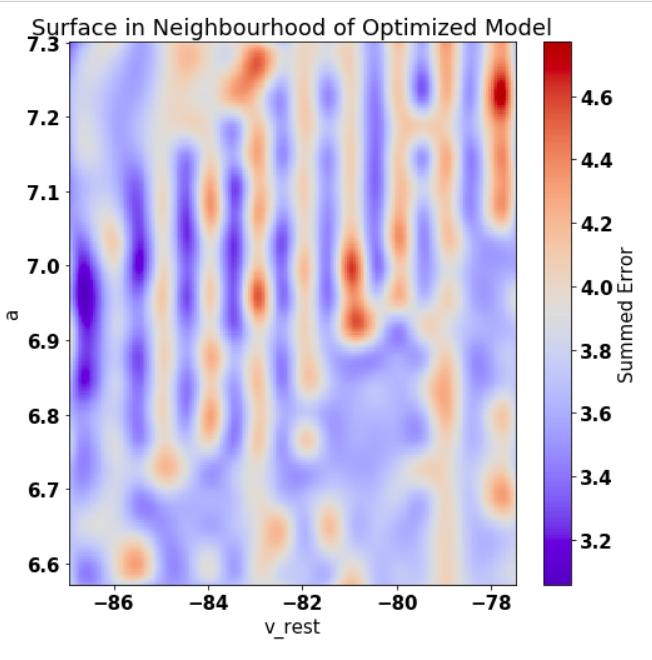
\includegraphics[scale=0.75]{figures/corrogations.png}
        \caption[A Complicated Error Surface]{\textbf{2D Cross-section of the Error Surface for an AdEx Model using EFEL Features.}
    Similar to Figure \ref{fig:constant_current} except using an AdEx model and all 14 EFEL features.
    As the approach for creating multispiking model fits also contained contingent tests, the error surface is complex and Rastrigin-like}
    \label{fig:real_problem_nontrivial_surface-1}
\end{figure}

%\begin{figure}
%    \centering
%    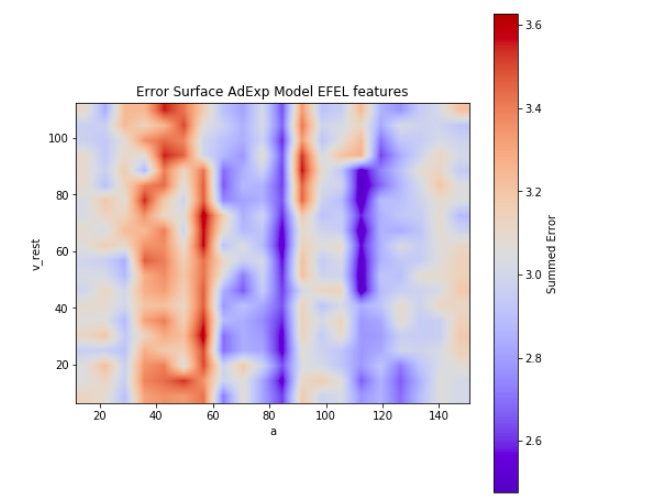
\includegraphics[scale=1.25]{figures/third_error_surface.png}
%    %\caption[Cliff ledge in 2D error surface]{Cliff ledge in 2D error surface}
%        \caption[Complex but not hopeless error surfaces]{Complex error surface %with alternating neighbouring ridges and valleys (ripples)}
%    \label{fig:real_problem_nontrivial_surface-2}
%\end{figure}

%%% . 
%The surprising complexity of these error surfaces did not become apparent to me until I had worked on this project for a few years. Its more complicated than that, I had evidence of complex surface since begining. We were dismissing as bug, as we did not conceptualize where these complex surfaces where coming from. Search slack, there are pictures of complex surfaces, since just after I started working on the project. I think the real problem is we were too confident in the first established NU tests, they where passing unit tests, which was good, but we should not have assumed they were conceptually sound to use in optimization.

%%%
I suspect that other pre-existing optimizers that aim to fit neuronal models are largely ignorant of the error surface they face.
In fact, without comprehensive data about the convergence rates of various competing approaches to optimization, we cannot now how efficiently each obtains its solutions, nor about alternative solutions that may have been missed.

Nonetheless, I am confident that genetic algorithms (in general) are preferable to to exhaustive search (which is impractical for all but the smallest models) and to gradient-descent-like approaches (due to the nature of the error surface).
However, successful optimization may benefit from periodic exhaustive, local grids searches of the parameters space near the optimized values, in order to evaluate whether the error surface was tractable in the first place.
% NB, this is harder to understand than the residual rheobase error idea.    
% dont need to share complexity with reader.
%Although not shown here a third case is worth describing, as this third test combination achieved many useful results: Izhikevich model at threshold virtual experiment. Constraints used:
%\begin{verbatim}
%Case1 + RheobaseTest,
%\end{verbatim}

\section{Satisficing Versus Optimizing}
%Genetic algorithms are favorable because they provide a good solution to the exploration/exploitation trade-off.
Unless hunting for a new prime number, few are willing to run compute jobs lasting for months, thus there are steeply limited budgets for exploring solution spaces. It therefore seems prudent to accept solutions which are are not optimal but are ``good enough", especially if these solutions can be obtained in a small fraction of the time.
Not all real neurons, even of the same nominal type, have identical properties, so perhaps we should embrace such variability in optimization results as well.
If the highest objective is to recover biologically plausible models, and many fitted models can easily meet this objective, then weaknesses in the ability of the optimizer to succeed in identifying the exact optimum in a very complex error surface can be tolerated.

Fortunately the coupling of Neuronunit to a Genetic Algorithm facilitates either optimizing or ``satisficing" as appropriate.
The term ``satisfice" means that a measured property is either deemed optimal or merely satisfactory \citep{simon1956rational}.
Although we may not know if a true optimum has been achieved, by using NeuronUnit in the evaluation, we can determine if the result is satisfactory enough, and then terminate optimization early.
This could be done by tracking the $\chi^2$ statistic during optimization and ending as soon as it drops below a certain level.

\section{Appropriate Optimization Constraints}
\subsection{Conflicting Optimization Constaints}
I identified multiple conflicts between features used for optimization.
In some cases, the conflicts may arise from limitations of the model, i.e. the model may lack the richness to lie at precisely the points in features space that some real neurons lie in.
However, I found that even for biophysically detailed neuron models, this limitation was sometimes still observed.
Thus, there must be some other source of these conflicts, which I identified as a conceptual pitfall in optimization: feature values computed from the mean of the corresponding features across many neurons (as in NeuroElectro) may not actually describe any real, single neuron (or in some cases any possible neuron). 
This was typical when combining the Rheobase, Input Resistance, and Time Constant, for example.

\subsection{Conflicts in Neuroelectro Measurements}
%%%
% 
%The NeuronUnit tests \emph{ThresholdTest},  \emph{SpikeHalfWidth}, and \emph{Spike Amplitude} were often incompatible with other tests due to the contingent discontinuity problem described in the previous section.
%By contrast, I experience few conflicts with \emph{FISlopeTest},  \emph{Capacitance},  \emph{Input Resistance}, and  \emph{Time Constant}.
%%%

%%
% Actually the two test sets above are compatible, the nuance is one set constitutes a reliable optimization guide, the other doesn't

% I found that you can still measure, 
%%  \emph{ThresholdTest},  \emph{SpikeHalfWidth}, and \emph{Spike Amplitude} after optimizing with the reliable guides and get satisfactory results for those measurements, but I anticipated that would confuse everyone too much.

% I did not want ambiguity the quality of fits on measurements that did not participate in guiding optimization.

% it is much easier to explain the quality of fits for metrics that did participate in optimization.


Membrane Time Constant measurements were consistently harder to use for guiding optimization, being incompatible with other features in almost all model types (including conductance based models, reduced models, and including all data types (NeuroElectro data and Allen Cell Types single experiment data).
This value is proportional to cell surface area, and it may be that cells taken from, for example, slices of different thicknesses have different capacitances but that this has minimal impact on other measurements.
Alternatively, most capacitance measurements could be in error due to recording pipette capacitance artifacts.
Regardless, when the membrane time constant was not included, optimized models were still able to behave in most other respects like their experimental counterparts

As discussed in section \ref{sec:parallel-rheobase} rheobase is strictly defined as the minimum current injection to evoke exactly one spike.
It does not fully define the FI curve, and there are an infinite number of FI curves that contain the points $(Rheobase^-, 0)$ and $(Rheobase^+, >0)$.

%%%
% I am not sure if I show this.
% I have (FIcurve + Rheobase)
% and I have (Rheobase+familiar tests)
%
% Actually maybe you are right.
% I had not thought about it in this way.
%%

Interestingly, if selecting only one suprathreshold feature to pair in optimization with the remaining physiological features, the FI slope was a better fit than the rheobase.
It may be that by considering the whole FI curve in optimization counter-intuitively makes optimization more flexible by allowing small misses on matching the rheobase in exchange for a better overall match to the remaining suprathreshold spike counts.

\subsection{Sufficient Optimization Constraints}
Avoiding conflict constraints, which tests are minimally sufficient to produce good optimization results?
Tests that worked within optimization:
Via \emph{Elephant} toolchain: FITests, Rheobase, Capacitance, Input Resistance, Time Constant, Resting Membrane Potential.
Via. 

\cite{druckmann2007novel} optimized neuron models using only suprathreshold stimuli by considering (1) spike rate; (2) an accommodation index; (3) latency to first spike;(4) average AP overshoot; (5) average depth of after hyperpolarization (AHP); and (6) average AP width.
However, when optimizing reduced neuron models, I found that the those 6 features measurements were insufficient for optimization, and additional constraints were required.
Overall, I found that the following features from the EFEL library were sufficient:
\begin{enumerate}
\item AHP-depth
\item all-ISI-values
\item Spikecount %$ (similar to rate)
\item adaptation-index
\item mean-AP-amplitude
\item min-voltage-between-spikes
\item minimum-voltage
\item peak-voltage
\item spike-half-width
\item time-to-first-spike
\item time-to-last-spike
\item voltage-base
\end{enumerate}

%\subsection{Exploting the FI Curve}
%There is visibly almost perfect  agreement between simulated and experiments and the optimized models, in the passive experimental conditions, and a close match for the spiking model behavior. There was a standard suite of tests if only spike-half-width, not spike-base-width. The Izhikevich models width as thus free to vary at the base, take that into account when eye balling the two graphs and you can see why almost binary match. EFEL does achieve spike width binary matching because it uses both half-width, and base-width. If you look at the last cells you can see I take a correlation matrix of the optimizers errors over its history. The idea is if it's normalized then I can sum the whole matrix and get a single scaler number to show how uncorrelated both error sets are over the GA evolution. 

%It was found that the elephant/neuroelectro-suite of NU tests don't fully constrain the spike width at the base of neuron action potential waveform. Since the base of the waveform was unconstrained, it was free to vary, half-spike-width is constrained, it is more appropriate to talk about variance explained of the spike snippet. $variance explained>0.95$ is a useful heuristic. Allowing some margin acknowledges that we shouldn't assume we have represented all waveform features that can vary. If you want $variance explained==1$   
%you could optimize using a variance explained 
%cost function, but we don't want to do that.
\section{Challenges of optimization}

\subsection{Ability of models to Fit NeuroElectro Literature statistics (NeuroElectro).}
Three classes of experimental measurements were used to fit models in conjunction with genetic algorithms. These consisted of four groups of eight neuroelectro observations, and four groups of Allen electrical measurements from single cells. And also a group of  $14$ different EFEL measurements that were obtained by sampling Allen Brain sweep Data.

When comparing generic single compartment models, to the BBP neocortical layer 5 neuron, one can see that there are often conflicts between Rheobase, FISlope and Time Constant mearurements. As a pattern the Multi compartment and single compartment conductance based models optimized in this work seemed to have trouble satisfying these three measurements at the same time.

See tables: \ref{tab:conductance_623960880}, \ref{tab:conductance_623893177}, \ref{tab:l5pc_table}


% It is worth noting that in both sets of measurements, the types of measurements that can guide optimization are significantly smaller subset of measurements of fitness criteria that can be evaluated on the final model.

%Final list of Elephant tests used to guide optimization: 
%\textbf{RheobaseTest}, InputResistanceTest, TimeConstantTest, CapacitanceTest, RestingPotentialTest.

In the Izhikevich model for each of the four different classes of experimental cell types, The optimizer finds a varied set of solutions, that are each within the range of empirical validity. Although overall neuronunit scores were found to be biologically plausible, the general pattern was that rheobase fitness was compromised as was required to bring all other measurements into a state of high fitnesss. % uncover models that were the fittest with respect to all the other fitness criteria.

Likewise In the single compartment conductance model, and the AdEx model, it was typically input resistance tests that experienced dominated solutions. 

As indicated by the $\chi^{2}$ statistic and $p$-$value$, many but not all model-test combinations were able approach empirical validity, the pathway to trading off, and letting fitness criteria dominate showed some consistency across model types.

%by all other fitness criteria in order for the optimizer to 
%\begin{comment}
%\end{comment}
%The EFEL measurements on Allen Data





%\item 

%\item Within a reasonable parameter range conductance based models are usually close to experimentally observed measurements.

%\section{A pattern to model fitting inability in Phenomenological Models.}
%* many reduced neural models are far from optimal at any point in parameter space. Optimizing does not significantly improve agreement. Optimizing does not bring model and experiment close to `Z=0`. There was some model to model variability however.

%\item There is an order of magnitude difference. Between agreement in Rheobase values between the conductance based models and the experimental models. 

%\end{itemize}

%\section{What does it mean.}
%\begin{itemize}

%\item  In methods I discussed an approach to verifying the optimizer.
%$-$ Specifically, we showed efficient optimizer convergence when constraints were derived from simulating experiments.

%When the optimizer setup is cogent because appropriate models and test combinations have been chosen, and because
%$N_{free_params} <= N_{constraints}$


%\item  In order to verify our approach we also re-implemented our code using BluePyOpts select best algorithm, and NSGA2.
%\end{itemize}

%Model constraint combinations give rise to differences in how correlated errors are during gene evolution. 

\section{Distinction of Optimization Approach From Other Approaches}
% This can be a fusion of your sections about multiobjective optimization, unit testing, and data integration (or whatever set of background items you think is fundamental to understanding the novelty of the work you have done).
The large-scale meta-analysis described here has not been performed previously. For the first time, a large number of cortical neuron and neuronal network models are available in the standardized NeuroML format. Although the Allen Institute for Brain Science modeling project and the Blue Brain project both rigorously analyzed their single cell models, to the best of my knowledge there has not been an overarching meta-analysis across different cell and network model sources.\\

Similarly, numerous modeling efforts have employed data-driven testing in model development workflows, but all these efforts have been based on non-standard ‘in-house’ model types and execution environments. In contrast, this work proposes to expand a pre-existing community driven, standardized model testing space, NeuronUnit, that supports model validation and re-use regardless of the model source. To date various NeuronUnit tests of action potential shape, electrical properties, and single cell morphologies exist; yet these tools are not unified. Some tests of network dynamics also currently exist; however, these tests are not integrated into a unified multiscale workflow. Although the work I describe only concerns single cell models in isolation, significantly, a unified workflow for exploring model data agreement would better locate errors in network behavior which are manifest at the network level but are caused by neuron-type models.

%\section{Stuff that belongs in results or discussion; please move there}%  Generalized Linear Integrate and Fire model\cite{teeter2018generalized} or
% EVERYTHING IN THE SECTION BELOW HERE BELONGS IN THE RESULTS OR DISCUSSION
We have used NeuronUnit to guide optimization by taking a flexible model types such as the Izhikevich model and then fitted these models using relevant experimental measurements inside our optimization frame work.

%As an example, select Best (IBEA) was used to optimize models in conjunction with data driven tests based on pooled data from NeuroElectro.org \cite{tripathy2014neuroelectro}. A variety of compact and fast single compartment models were used to explore model optimization. Figure 4 demonstrates test error at the beginning of the optimization process for models with randomly sampled parameters and the smaller error following optimization. Figure 5 shows the evolution of the error during the optimization process\\
%\\


Optimized neuron models may vary from their experimental counterparts for several reasons. In the appendix generally, there are multiple tables that show that optimizing models with respect to the rheobase fits comes into conflict with minimizing with respect to input resistance. The solution to the optimization problem consists of two sets of model parameters, which can resolve this conflict differently. Examining the experimental data that these tests were derived from suddenly becomes important. By examining the data, we can see if the rheobase currents and the distributions of input resistance are bi-modal and uniformly distributed. If the data is treated as uni-modal, and the uni-modal mean is used to optimize then the model, then the model is not able to satisfy both constraints simultaneously. In this case, the measurements don’t correspond to neuron data, and the model can’t produce the artificial behavior. When comparing complex data and simple models we find that solutions are better represented using a combination of two optimization solutions.\\

Another potential issue to consider when evaluating the scientific merit of a model is that neurons may have different behaviors under different stimulation paradigms. It might be appropriate to compare modeled behavior against measurements specific to each of two or more distinct modes. In this case, when optimizing single cell models, it’s appropriate to accept a solution set, rather than a single solution. For example, the cerebellar Purkinje cell is sensitive to intricately patterned dendrite input current combinations. Depending on a cell’s recent history of synaptic stimulation, a Purkinje cell may toggle between coincidence detection and integration modes \cite{ratte2013impact}.

The are several valid instances when the complete three dimensional form of a neuron (and the 3D form of a network) is an integral part of a brain simulation, such as in the Blue Brain somato-sensory cortex model \cite{markram2006blue} and the Allen Institute \emph{V1} model \cite{billeh2020systematic}, The Allen Institute \emph{V1} simulation was improved by encasing a "core" of biophysically accurate models inside a "shell" of simple fast and reduced GLIF models. Results from this work suggests that pre-existing large scale brain simulations might be further improved by including a shell of AdEx or Izhikevich models.% The literature states only GLIF models, I am not proposing what they should do, only what I have read about.

%Izhikevich, GLIF, or Adaptive Exponential Integrate and Fire models.\\ 

Encasing a core of complex models inside a shell of simplified models mitigates a harmful edge effect. The problem is that simulations concern sub divisions of brain tissue and without intervention the act of making a subdivision severe synaptic inputs. All published highly detailed simulations to date, have necessitated the simulation of severed volumes of tissue, and this creates another problem to manage.\\
%There is a core of models of realistic models who are missing a substantial number of "extrinsic" synaptic inputs. Many synaptic inputs are severed by the process of making a subdivision.
\subsubsection{Merits of Extending Biophysical Accurate Simulations by Including Reduced Models}
Almost all cortical neurons experience ``tonic" synaptic input and these tonic inputs originate from neurons from a different part of the brain. One strategy for handling missing inputs to the region of interest, is to simply model spike trains for each input synapse. This approach to modelling synapses is called a Point Process, or a spike train surrogate. Modern programming languages have tools that can make the synthesis of statistically similar spike trains easy and convenient. One big problem with this approach is that such surrogate spike trains are impervious to Local Field Potential (LFP) analysis, as point processes fail to model current flow in the soma and dendrites. Because synapse activation is predicted using stochastic models, the mechanistic reasons that lead to firing are opaque in the point process model, likely there will be no physical sequence of cause and effect steps to explain synapse firing. Although point process modelling sounds potentially simple, point process models can in fact be very elaborate, and therefore they may be slow to execute. Reduced models by contrast, are potentially fast to evaluate, their mechanisms are transparent and have some phenomenological relationship to membrane physics. Reduced models can also produce somatic currents. Somatic currents may facilitate the imputation of dendritic current. Modelled somatic currents can therefore be read-out and measured in network models of Local Field Potential.
%assumes that post synaptic neurons are mainly influenced by the firing rate of inputs, if they pre-synaptic neurons are actually conveying important code words via exact interspike intervals, a statistical approach to modelling spike trains would not do.\\

%than generating only psuedo random timed inputs to synapses, 
In the case of the Allen Institute Model, if the region of interest V1 is a "core" of realistic neurons. That is a kernel of realistic neurons encased by a shell of less realistic neurons. Inputs to V1 also come from the outer encasement of neurons. It is therefore of interest if these external GLIF models can or should be substituted with optimized Izhikivich and AdEx models, in case substiting GLIF for Adex results in an overall more realistic network simulation. In that case, even the external shell of simulation could experience a marginal improvement in accuracy. In network models there are benefits of reduced models over the use of a point process or a spike train surrogate.\\

% benefits: interpretability, transparent function, has current so contributes to LFP

One of these benefits is that the firing of reduced neural models can be made to be causal, such that its spike times are not just what statistically matches missing models. Furthermore reduced models can still participate in networks, reduced models can become disconnected or participate in an dynamic assembly. Realistic levels of plasticity of the modelled network is more possible with included reduced models, than statistical surrogates of those models.

Furthermore Izhikevitch and AdExp models are commonly utilized in neuromorphic spiking neural networks in artificial intelligence and bio medical modelling contexts.
%archictecture.

%\subitem 
optimization is an interaction between models and constraints which guides a fitting process. Not all neural models are equally flexible.  
%\item  
Both the choice of constraining equations, and the choice of neural models must be favorable in order for models to be fitted to data.
%\item 
%\subitem 
if the combination of models and constraints is bad, then then a tractible error surface will not result.  

%\subsubitem 
Unfortunately, it is not always possible to know without trying which combinations of A: models, and B, constraints will lead a tractable error surface, however a nicely smooth manifold surface with only minor oscillations is preferable

%that a Genetic Algorithms can use to find a global solution to. As an example consider  

\subsection{Optimizing Multispiking Behavior}

When using Allen experimental data to create multi-spiking tests, there was the potential to more tightly constrain model behavior. In order to evaluate the goodness of fit models the $\chi^{2}$ statistic could no longer be used, instead one could compute the 'variance explained ratio' between the allen institute experimental sweep and the optimized models sweep to a comparable current injection.

and there is also the potential to check the variance explained ratio of tests. In such a multispiking paradigm the highest possible variance explained ratio of approx $1$. 


There is visibly almost perfect  agreement between simulated and experiments and the optimized models, in the passive experimental conditions, and a close match for the spiking model behavior. There was a standard suite of tests if only spike-half-width, not spike-base-width. The Izhikevich models width as thus free to vary at the base, take that into account when eye balling the two graphs and you can see why almost binary match. EFEL does achieve spike width binary matching because it uses both half-width, and base-width. If you look at the last cells you can see I take a correlation matrix of the optimizers errors over its history. The idea is if it's normalized then I can sum the whole matrix and get a single scaler number to show how uncorrelated both error sets are over the GA evolution. 

It was found that the elephant/neuroelectro-suite of NU tests don't fully constrain the spike width at the base of neuron action potential waveform. Since the base of the waveform was unconstrained, it was free to vary, half-spike-width is constrained, it is more appropriate to talk about variance explained of the spike snippet. $variance explained>0.95$ is a useful heuristic. Allowing some margin acknowledges that we shouldn't assume we have represented all waveform features that can vary. If you want $variance explained==1$   
you could optimize using a variance explained 
cost function, but we don't want to do that.


\subsubsection{Persistently Incompatibility Tests: Trends and Patterns}

Time Constant measurements were consistently harder to fit, and where often incompatible, in almost or all model types (including conductance based models, reduced models, and including all data types (NeuroElectro data, and Allen cell-types single experiment data). When the membrane time constant was mismatched, this didn't seem to be of much consequence to other membrane timing measurements in the cell, for instance membrane capacitance, spike widths and spike-thresholds could still be accurate. Frequently mismatched membrane time constants suggests either one of two possibilities: Either our method for measuring membrane time constant is wrong, and is off by a factor of 10, or, model builders write equations that are founded on electrical properties that are preference AP features and electrical properties slightly that don't involve the membrane time constant.

Interestingly there was better compatibility between firing rate versus current (FISlope) and the remainder of the electrical observations (where the remaining measurements tended to agree well with each other), than between rheobase and the same measurements. Compatibility was also experienced between the FISlope and Rheobase tests, so two natural clusters of tests that emerged are: FI curve properties, versus the other electrical properties.

As discussed in the methods \ref{sec:parallel-rheobase} Rheobase is defined as the minimum current injection to evoke exactly one spike, therefore, rheobase can sensibly be drawn onto the FISlope for an experimental cell.. The FI line is not fully defined by the slope, as the slope defines the lines gradient but not its bias, however, because the rheobase value falls on the FI-curve, it intersects with the line which has both the bias and the slope of the FI curve. 

%Taken together,
In the situation where, FI-slope is matched, other electrical measurements match, but rheobase is mismatched; when electrical properties agree with the FI-slope but not the rheobase, this suggests, that the overall linear relationship is correct but the exact quantity of current that biases the FIslope is wrong in models. One reason for this could be due to the difference between modelled resistance, and material resistance in neurons. Another reason, might be because, in the virtual experiments where I measured rheobase, I only used a single value of integration time that was a $1$ second duration,  square current pulse, but experiments could have used either shorter times (stronger currents needed to evoke single spike), or longer integration times (less current needed to evoke a spike).


\subsubsection{A Fitted model may not generalize to injections at higher or lower current stimulus, Unless the model is fitted with constraints informed by those different experiments}
As discussed above, the true FI curve is described by a gradient and a bias. When one fits to both the slope and the bias of the FI curve, it means that the model will at least be able to recapitulate the right number of spikes for  a given current strength. %Although this does not necessarily mean that the shapes of the each individual spike will agree between model and experiment. 
% important for network modellers as I discuss elsewhere.

%Preserving 
%
%that required current injection increases causes proportionate firing rate increase, 
% suggesting No, it cannot reduced neuronal models are only okay at fitting one sweep at a time.

The utility of the Rheobase approach is to demonstrate a work flow. Its possible that some researchers are interested in modelling single spiking behavior efficiently, however, in the context of network simulations, one may be better of fitting to a multispiking sweep.

In reduced neuronal It was found that the electrical properties of cells:
 (Rheobase, input resistance, membrane time constant,Resting Potential, Capicitance)

 did not encode the above threshold spiking behavior of neurons, when neurons were undergoing a multispiking stimulus regime.

 forinstance in Allen cell $482493761$ injecting a current of 
 specified by:
 \begin{minted}{python}
 from quantities import pA, ms
 current = {'amplitude':110*pA,'duration':1100*ms,'delay':100*ms}
 \end{minted}
 should elicit a spike count of $3$, in an optimized Izhikevich model that has good agreement with all values except for Rheobase these values it produces $33$ spikes.

One can imagine that in cells that have been optimized to rheobase only, that current spike count relationship might be more  accurate and faithful to the experiment.

In cell 471819401 , $290 pA$ causes $20$ spikes,
in the optimized Adaptive Exponential model $290$
specified by:
%\begin{lstlisting}[language=python]

\begin{minted}{python}
 from quantities import pA, ms
current = {'amplitude': 290*pA,
           'duration': 1100*ms,
           'delay': 100*ms}
\end{minted}
%\end{lstlisting}

caused only $5$ spikes. and in the Izhikevich model $59$



\begin{table}
\centering
\begin{tabular}{lllll}
            & RheobaseTest & TimeConstantTest & RestingPotentialtest & InputResistanceTest  \\
Observation & 70.0 pA      & 24.4 ms          & -71.6 mV             & 132.0 MOhm           \\
Prediction  & 234.67 pA    & 31.31 ms         & -72.08 mV            & 130.26 MOhm          \\
Z-score     & 3.98         & 0.09             & 0~                   & 0.01                
\end{tabular}
\end{table}


Another way of writing this is that fitting a model to electrical properties of cells, does not
guarantee that the cell is fitted to suprathreshold behavior, at current injection virtual experiments with larger amounts of injected current.
A model fitted to one "sweep" is a model of only that sweep. 

If you apply the sweep fitted model to a different current injection value, you will not get the expected waveform shape fitted.
because even though one may have optimized to the shape of a single spike, and the membrane time constant, and input resistance should have a bearing
 on spike width and spike height respectively. Since spike width is dependant on membrane time constant, and input resistance, you 
 would expect that spike frequency and therefore firing rate, should be proportionately related to 
 to the membrane spike width, and therefore membrane capacitance. However, in reduced neuronal models, this was found
 to be not strictly the case.

 The Rheobase value is the biggest determinant of how current injection values map onto spike counts.


 Arguably then only the rheobase current injection value is important for fitting to Reduced Neuronal Models in order to make networks of Reduced Neuronal cells behave more realistically.
 It is unclear, however, what the relationship is between synaptic current and electrode current. Synaptic current is distributed, but electrode current is focused on a single point.
 If both are distal to the axon hillock, both synaptic current, and injected currents may behave in a similar way.


 These model parameters do not encode the spike frequency.
you didn't optimize to the spike count at different injection values.

Therefore in order to make realistic network models that make use of reduced models, 
one should have a firing rate, and some sweep data, of cellular behavior with the same spike frequency.
one can then fit simple multi-spiking waveform measurements to the models.

Surprisingly some types of spiking information, like spike rate, and multispiking height, spike adaption.
Are easier for reduced models to fit. I show this in some simulated data, virtual experiments.

% With spike counts, and spike frequencies, 

\subsubsection{Future Work}
Because of the benefits of the NeuroML model specification, data fitted models should be downloadable in a NeuroML format. NeuroML is simulator agnostic, descriptions of the optimized models will be more shareable, if they are not pinned down to their numba-python implementation. NeuroML models should can be deployabled by any mainstream simulator. %When model parameters are inserted into NeuroML cell model definitions, NeuroML encoded models become operational. These NeuroML encodings will if possible be uploaded into NeuroML-DB, where they will be more readily find-able by the neuron modelling community
% Such files can be used as network components, and they confidently utilized and exchanged, as such files represent a higher degree of rigor. Since there are two classes of model fits, some models are better suited fitted to network modelling and others are better suited to single cell modelling, this is because, by fitting cell models to FI curves, a lot of other realistic electrical behavior that is incompatible with the FI fit diminishes.

At least for the Izhikevich, model links to the reference models, can also be provided.
%\section{One Feature Extraction Package to Rule Them All}
\section{Largest Possible Survey of Features}
The NeuronUnit core, the Electrophysiology Feature Extraction Library \citep{EFEL}) EFEL, the Allen SDK, and the tests derived from \citep{druckmann2008evaluating} all contain independently written algorithms for computing features from simulated membrane potentials.
In some cases, the same feature (e.g. action potential threshold) is computed in many different ways across these feature extraction libraries.
All compute the threshold by first taking the first difference of the membrane potential, but they differ in subsequent steps, for example what value the first difference must reach to be considered at or beyond threshold.
This is inconvenient, but one can simply select one (or more) of the alternatives and apply it consistently.
More troubling are the cases where these algorithms differ in the stimulus used to generate the feature.
For example, the suprathreshold tests of \citep{druckmann2008evaluating} are based on a multiple of rheobase (e.g. $1.5\times$ or $3\times$), whereas those used by The Allen Insitute are based on additive increments from rheobase (e.g. +20 pA or +40 pA).
This means that cannot simply be applied to the same membrane potential trace, as those who collected the experimental data are likely to have chosen either multiples or additive increments of rheobase, but not both, depending on which lab they happen to work for.

As discussed in the Methods, I wrote code to restructure the Allen Cell Types and Blue Brain Project data sets, sorting traces into (approximate) multiples of rheobase, and the interpolating to select the sweep (in one data set) that is most appropriate for computing the feature defined in an otherwise-incompatible feature library.
In this way I was able to generate the same set of features from distinct datasets, even those that had use different stimuli.
%To make these conflicting lab protocols interoperable I impute 1.5 $\times$ and 3 $\times$ rheobase where it was not provided by finding the stimulus sweep pair that is the closest approximation. In this way I find the nearest traces to those predicted values in the Allen and BBP collections of sweeps.

One can conceive of more mathematically savvy types of imputation, and these could be the basis for future work.
If a more robust form of imputation was achieve, it could act as a Rosetta stone to link all the above feature extraction libraries together, allowing nearly any \emph{in vitro} dataset that is being collected to be used to produce a canonical and universal set of features for model optimization.
%that is what I mean when I write imposing a new organisation on the sweep data.

% It may be possible to generate predicted features from one stimulus convention based on observed features from the other, allowing imputation of a full set of features across all algorithms, but this is beyond the scope of my thesis work. ISNT THIS WHAT I DID IN SOMEWAYS? IF I COULDN"T COMPARE ACROSS LAB PROTOCALS THEN THE ANALYSIS I DID WAS POINTLESS WAS IT NOT?

\section{Cross-Validation for Feature Selection: One Feature Set to Rule Them All}
The features identified during multivariate analysis utlilized the entire collection of models, data, and stimuli.
By contrast, a machine learning approach would have held out some of these for cross-validation, checking to see whether the features identified on a training set were in fact that features that best cluster, discriminate, or simply explain variance in the a held-out set of models and data.
For example, future work could identify a canonical set of stimuli and features fitness criteria, criteria that can train models to best satisfy multiple experimental protocols, rather than just one particular experiment.
These features would be shuffled (using stratification according to the stimuli that generated them) the objectives into ``train" and ``test" sets.
Cross-Validation may provide a strategy for dealing with conflicted features, such as the input resistance test.
If a trained model failed to score remotely well on such a test, this might identify that the model was overfit or simply that the test was unsatisfiable (given a model fit to the other tests).
This would allow for quick identification of which test combinations cannot work in practice, while also producing more generalizable models.

\section{Which is the Best Model Class for Producing Optimized Reduced Models?}
In previous spike-time prediction competitions \citep{incf_multi}, multi-time-scale variants of the AdEx model performed best.
It also had an admirable performance here, however the Izhikevich model was the overall winner.

Considering only features of at or below threshold spiking, the features that where used to get results below come from the tables 

By consulting tables: (\ref{tab:main_chi2},\ref{tab:HH_chi2}), and aggregating scores using python pandas, and averaging across $\chi^{2}$ statistics (which reflected 12 tests) for all neuron types, the Izhikevich model had the lowest mean $\chi^{2}$ (AdExp=$28.55$; Izhikevich=$1.39$), and the highest average $p-value$.
However, the Izhikevich model did not have the lowest $\chi^{2}$ for every cell type (see the Appendix for details).
%.when regarding each data set as a novel contest, the Adaptive Exponential lost to the Izhikevich model on two or more data sets see appendix \ref{appendix}.
%Adexp $28.55$ versus 
%Izhikevich $1.39$


The AdEx model suffered from its performance on the Olfactory Bulb Mitral Cell and the Cerebellum Purkinje cell (two of the largest cells types that were optimized). 
However, if you remove these two cells, and then judge the optimized models for the remaining cell types, the AdEx model is the winner by $\chi^{2}$ (AdExp=$0.51$; Izhikevich=$0.99$).

When consulting some of the traces for fitted models, it seemed as if either the AdExp and Izhikevich models lack the flexibility to model diverse cortical neuron activity, or the NeuroElectro data was difficult to fit.

% In summary, the AdEx model is well-suited to cortical neuron types, but the Izhikevich model may have the flexibility to model the entire brain.
%The GLIF model was worse than both of the other model classes, and was limited in the same way as the AdEx model.


Consider two sets of features: {RheobaseTest, TimeConstantTest, RestingPotentialTest, InputResistanceTest} or {RheobaseTest, FITest}. If you consider only the Allen Cell Types data (all cortical neurons), with these two sets of features, the GLIF model is associated with $\chi^{2}=1.0$; however, if you consider other neurons (and tests), the mean $\chi^{2}$ value jumps to $364.2$. The GLIF model was able to recapitulate the FI curve slope exactly; however, this caused conflicts with the ability to fit the time constant and rheobase. Even when the GLIF model was able to optimize cells to be within a biologically plausible range, simulation was slow and the quality of fits was not astounding. It is unclear why anyone would choose to use this model outside of a very narrow range of applications.

Why did the Izhikevich model perform best? I hypothesized that this was related to its broader coverage of dynamical regimes (as shown in \citep{izhikevich2003simple}).
To test this, I asked how many of these dozens of regimes were ``occupied" by the optimization solutions obtained here. Specific optimization results (Section \ref{sec:appendix}). I developed the Izhikevich model, such that regime type was an explicit integer model parameter. Numbers 3-7 encoded regime types 1-7, where regimes 1,2,3 follow identical governing equations and so do not require unique numeric identifiers. I show that all but one of these regimes were occupied except for one associated with the activity of a dorsal LGN thalamocortical cell.
The ones associated with a barrel cortex low-threshold spiking (LTS) interneuron and a Layer 5 visual cortex fast-spiking (FS) interneuron were occupied the most often. 
%Regimes $1-3$ in this case representing the "regular-spiking" regime. A little surprisingly the regimes $1-3$ were only used in one fit Allen specimen $id-623960880$.


\section{Parameter Boundaries}
The error surface explored by the optimizer cannot extend infinitely far in all directions.
It must be initialized with boundaries that contain plausible parameter values.
If these boundaries are too narrow, they may exclude the optimal set of parameter values.
However, if they are too wide, then parameter sets that produce models well outside the range of biological plausibility will be produced.
Such implausible models undermine the assumptions of the features being calculated, and result in discontinuous or otherwise uninformative error surfaces where the optimizer wastes time exploring and may struggle to escape.
An example of parameter boundaries from the literature is shown in Figure \ref{fig:best_at_edge_2}.

\begin{figure}
    \centering
    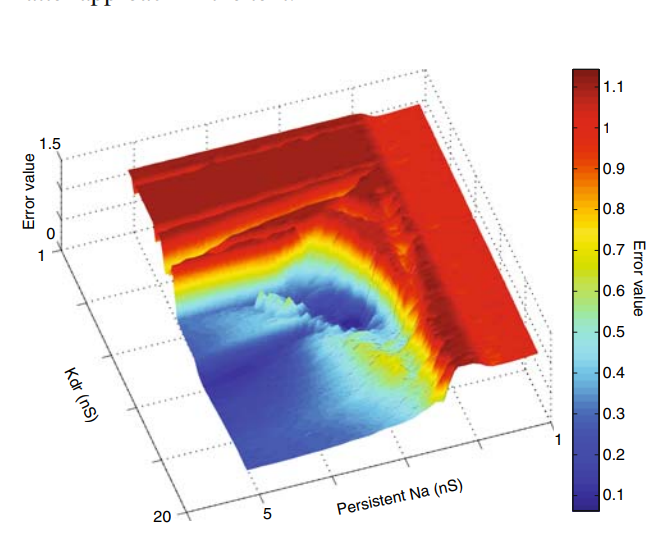
\includegraphics[scale=0.65]{figures/cliff.png}
    \caption[A Plot of a Cliff Ledge Framing a 2D Error Surface]{\textbf{Parameter Boundaries Can Frame the Search Space.}
    This error surface plot (from \cite{van2007neurofitter,van2008automated})
    shows how model/data agreement varies as two conductances from a biophysically-realistic conductance-based model are varied.
    The large error values for $Na<2$ and $Kdr<2$ suggest that the decision not to search below the value 1 for either of these parameter was reasonable.
    Similar grid searches could help to justify the parameter boundaries for optimization problems, provided that they can be conducted at low computational cost relative to optimization itself.}
    \label{fig:best_at_edge_1}
\end{figure}

For example, some parameter sets may cause a divergence in either the simulated membrane potential or in the features extracted from it.
This will be encoded as either ``not a number" (NaN) or $\inf$.
A single (NaN) or $\inf$ can infect the entire multiobjective function (i.e. any sum with $\inf$ will be $\inf$).
Because the optimizer can only succeed when it can distinguish better parameter sets from worse parameter sets, any chromosomes that get stuck in regions of parameter space with (NaN) or $\inf$ may not escape, even through mutation or crossover.
The error surface is locally ``flat" in a sense, and thus uninformative.
In order for the optimizer to survive the existence of such regions, the population size must be sufficiently large that a large number of chromosomes will avoid being initialized there.

In the opposite case, consider what might happen if the parameter boundaries are too narrow.
Figure \ref{fig:best_at_edge_2} shows another case from the literature, and in this case the global minimum error is positioned in a deep and narrow well.
It would be easy to have chosen parameter boundaries that miss this well entirely, resulting in a failure to obtain the optimal parameter set. 

\begin{figure}
    \centering
    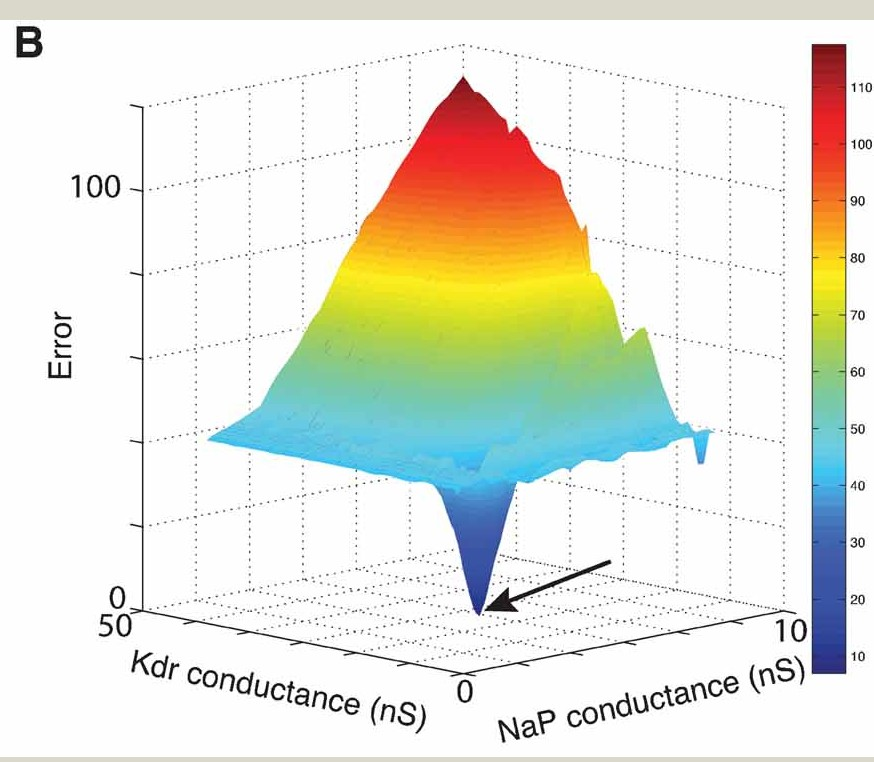
\includegraphics[scale=0.65]{figures/fninf-01-001-g009.jpg}
    \caption[A Challenging Location for the Optimal Value]{\textbf{A Challenging Location for the Optimal Value}.
    Again from \cite{van2008automated} I show an example of well-chosen parameter boundaries.
    These boundaries enclose the (narrow, deep) global minimum.
    Notably, choosing to explore only one quadrant of this space, where the error is roughly invariant to the parameter values, would have led to missing this global minimum entirely.}
    \label{fig:best_at_edge_2}
\end{figure}

A possible solution the problems above is to employ algorithms that peek beyond parameter boundaries and reports back on model stability.
This would be done only sparingly (otherwise it is equivalent to simply expanding the boundaries).
%In this manner one can do obtain the maximum parameter boundaries in an supervised computer algorithm, however, model equations used here, do exhibit some higher order sensitivity by changing a second intermediate parameter. Very quickly this approach to finding the maximum scope of a parameter may begin to look like exhaustive search.

%Another programmatic approach is to use a wide variety of models and tests, and to accept that for some model-test combinations, for some regions of parameter space, genetic algorithms are at worst randomly stumbling upon satisfactory solutions, and at best efficiently learning the optima solutions.


%The genetic algorithm
%As discussed, model-solution instability can occur when the optimizer samples model parameters that are outside of the models intended scope, or when a model returns a nan value inside its intended scope. It is tempting to think of 

%Usually these flat cliffs that neatly encase the error hyper volume like in the figure below \ref{fig:cliff} (and as described above).

% Not helpful for audiance to understand.
%unfortunately however, because each model has a large number of parameters typically $>10$, any particular model instance, only one of these parameters need be evaluating an unstable model when exceeding a margin, the rest of the parameters may be in the middle of their range, and so such a ledge may mostly be experienced as a hyper dimensional "tower", this tower could actually be experienced in the middle of parameter space in 10 out of 11 parameters, while still being on at the edge for only the 11th parameter. The unfortunate consequence of such towers is to lesion in the middle of parameter space inhibits the migration of chromosomes between regions. 

%From one perspective, the genetic algorithm is robust, and any middle region discontinuities are usually only a temporary hindrance that slows down learning without stopping it completely. From another perspective there are is only a small number of samples that occur inside the GA framework, and it would be better if the occurrence of lesions in the middle of the error surface were reduced to maximize the informativeness of every precious sample. 

%The major strategy for circumvent unnecessary ridges and towers is to pick and chose error functions sparingly and to assess results in a piecemeal basis. Utilizing a "sparing" inclusion policy will have to occur despite the large conflicting incentive to employ as many objective functions as possible.

% Picking the right objective functions will likely involve favoring a-posteri evidence over a-priori arguments about which errors "should" work best. 

%the majority of samples in the middle of the error space.

%To supplement figures from the literature, here I include some figures from problems encountered in this work.

%Although we are considering single points, and not surfaces, very often if a point is unstable, its neighbours are also unstable, in this way points of instability tend to be a constituents of larger regions of surface that add up to towers, cliffs and ledges such as those in seen here {fig:cliff}.

%One or more cliffs or towers situated in the middle of the error surface, poses problems for efficient optimization, where genes learn the general shape of an error surface. %Such cliffs and ledges will mislead the optimizer and they will act exactly like the ripples discussed briefly before in this work.

%Type \textbf{2}: While some towers can be circumvented by choosing slimmer parameter margins, other ledges and ripples of these ledges are implied by the types of model and test combinations. Rather than being avoidable, they are a feature of the complex problem that the optimizer is tasked with solving.

%Forinstance, in bursting regimes of the Izhikevich model, where models deliberately produce close to unstable limit cycles. When surpassing the threshold to cause spiking, the slightest increment of current  will illicit not a single spike but a burst of ten.

%Rheobase values will be undetermined, because the a  current injection value to that causes only one spike does not exist. The models rheobase value will be assigned to 100, and a tower will punctuate, the error surface possibly in the middle of the Izhikevich parameter hypervolume. The experience of sampling this tower, will visible in evaluation of the  algorithms learning performance. It will likely appear as a one or several unexpected peaks late in the genetic algorithms learning. Also this tower may act to lesion error surface, and to inhibit the movement of chromosomes across the solution space.

%This means that even under the most tractible conditions when evaluating the performance of genetic algorithm learning, the rapidity of genetic convergence will vary depending on which constraints are chosen, and the regime that the neuronal model is currently sampling from (the models parameters). There will be regions of genetic learning when models will encode high local pockets of error, or "towers" in the middle of the hyper-volume, and if these towers are significantly wide or densely populated, the genetic algorithms learning will be visibly diminished to a random sampling algorithm. What is more, these discontinuties under some circumstances may act to lesion error surfaces and inhibit migration of models from side to side. Movement over cliffs of course will still ultimately occur due to stochastic pressure in gene mutation.


\section{Future Work}
\subsection{Fixing Currents}
Here I identified a problem of contingent tests, which cause sometimes intractable defects in the error surface.
This could be solved by specifying all injected currents in advance and fitting directly to the entire FI curve.
Having been fit, features that are defined near rheobase (such as spike threshold) should then be computed at a pre-determined current.
%Despite there being negative consequences of this error for the signal sources tat guide optimization, there is still a mandate for models with different preferred currents to participate in testing. Preferred current searches are easily separable from Genetic Algorithms, meaning that a preferred current search can occur in an isolated part of a different algorithm where it will not act as the basis for electrical measurements. Over the course of a genetic algorithms search a fixed current can be applied to all models, allowing electrical measurements to be grounded to a stable value. Genetic algorithms can easily be nested inside each other, its easy to conceive of a situation, where an inner GA evaluates model fitness according to fixed currents, and an outer GA changes the fixed current that is used on each inner GA batch.
%The result of such a process should be a collection of optimized cells, that where obtained according to a different fixed current injection strength. %If one optimized model is clearly better, then two things about the model are revealed. What is the cell models preferred current, and what how well did it fit the tests? 
%This scheme is also different in that it treats current injection strength as a model parameter, and not a emergent feature of the model.

%cause of this finite precision error, 
%When model parameters are inserted into NeuroML cell model definitions, NeuroML encoded models become operational. These NeuroML encodings will if possible be uploaded into NeuroML-DB, where they will be more readily find-able by the neuron modelling community
% Such files can be used as network components, and they confidently utilized and exchanged, as such files represent a higher degree of rigor. Since there are two classes of model fits, some models are better suited fitted to network modelling and others are better suited to single cell modelling, this is because, by fitting cell models to FI curves, a lot of other realistic electrical behavior that is incompatible with the FI fit diminishes.

%At least for the Izhikevich, model links to the reference models, can also be provided.
\subsection{Model Exchange}
The NeuroML model exchange format \citep{gleeson2010neuroml} offers a portable, simulator agnostic, description of a neuron model including its parameters.
A logical next step is to capture the results of optimization and use them to specify these parameters, resulting in an optimized model that anyone can use.

\subsection{Embedding Models}
Reduced models could be especially valuable when embedded into a larger network that simulated a part of the brain
%, such as in the Blue Brain Project \cite{markram2006blue} and the Allen Institute \emph{V1} model 
The Allen Institute followed an approach like, encasing a "core" of biophysically accurate models inside a "shell" of surrounding, simple, fast and reduced GLIF models \citep{billeh2020systematic}.
%Results from this work suggests that pre-existing large scale brain simulations might be further improved by including a shell of AdEx or Izhikevich models.% The literature states only GLIF models, I am not proposing what they should do, only what I have read about.
%Izhikevich, GLIF, or Adaptive Exponential Integrate and Fire models.\\ 
Since almost all cortical neurons experience ``tonic" synaptic input, often originating from outside of the local circuit, such reduced models could be used to provide this input in a semi-realistic way, even as the neurons they target are simulated in greater detail.
Currently, this is often handled statistically rather than dynamically, by simulating some number of point processes to provide such input.
However, this makes strong assumptions about the nature of that input, and does not allow it to change dynamically the way it would if it originated from an actual neuronal or network simulation.
Reduced models can also be extended to include multiple compartments, allowing Local Field Potential (LFP) analysis to be included among the benefits of such an approach to network modeling.
The statistical approach also severs the link between cause and effect, and does not have any phenomenological relationship to known physics.
Finally, Izhikevitch and AdExp models are commonly utilized in neuromorphic spiking neural networks in artificial intelligence and biomedical modelling contexts, suggesting that their optimization in software could result in superior implementations of identified cell types in hardware.


%than generating only psuedo random timed inputs to synapses, 
%In the case of the Allen Institute Model, if the region of interest V1 is a "core" of realistic neurons. That is a kernel of realistic neurons encased by a shell of less realistic neurons. Inputs to V1 also come from the outer encasement of neurons. It is therefore of interest if these external GLIF models can or should be substituted with optimized Izhikivich and AdEx models, in case substiting GLIF for Adex results in an overall more realistic network simulation. In that case, even the external shell of simulation could experience a marginal improvement in accuracy. In network models there are benefits of reduced models over the use of a point process or a spike train surrogate.\\

% benefits: interpretability, transparent function, has current so contributes to LFP

%One of these benefits is that the firing of reduced neural models can be made to be causal, such that its spike times are not just what statistically matches missing models. Furthermore reduced models can still participate in networks, reduced models can become disconnected or participate in an dynamic assembly. Realistic levels of plasticity of the modelled network is more possible with included reduced models, than statistical surrogates of those models.


%Encasing a core of complex models inside a shell of simplified models mitigates a harmful edge effect. The problem is that simulations concern sub divisions of brain tissue and without intervention the act of making a subdivision severe synaptic inputs. All published highly detailed simulations to date, have necessitated the simulation of severed volumes of tissue, and this creates another problem to manage.\\